\documentclass[a4paper]{article}
\usepackage[top=1.7cm, bottom=2.5cm, left=1.7cm, right=1.7cm]{geometry}
\usepackage{parskip}
\usepackage{graphicx}
\usepackage{amsmath}
\usepackage{amsfonts}
\usepackage{amssymb}
\usepackage{hyperref}
\usepackage{listings}
\usepackage{epsf}
\usepackage{float}

\title{MA3505 Multivariate Statistics Project 1}
\date{\today}

\begin{document}
\maketitle


\section{Introduction and exploratory data analysis for the variables.}


\section{Analysis to answer each research question}

\subsection{Question 1}

\newpage
\subsection{Question 2}

\begin{lstlisting}[frame=single]
model2 = lm(cbind(chol, thaldur, thaltime, met, thalach, thalrest, tpeakbps,
		tpeakbpd, trestbpd, oldpeak, rldv5, rldv5e) ~ proto + restecg + dig
		+ prop + nitr + pro + diuretic, data=datall)
\end{lstlisting}

Using the above code I created the necessary multivariate regression model.
I was able to use this model to get the following table of coefficients:
\lstinputlisting[frame=single]{Q2_output/Q2_1.txt}
However this is not very useful, so I used the \textbf{summary()} function to
enable me to achieve a more detailed view of my analysis. Below I have tried
my best to explain the detailed view for each response variable.

\newpage
\lstinputlisting[frame=single]{Q2_output/Q2_2_1.txt}
From the table above we can see that the predictor that had the most
affect in the value of the \textbf{chol} response was \textbf{proto}. As
\textit{chol} refers to the amount of cholesterol in a person's system and
\textit{proto} refers to the type of exercise that they do, it is not a major
surprise that this is the most important as in theory the higher the intensity
of the your exercise program the lower your cholesterol will be. The second most
important variable is \textbf{pro}; this is an indicator variable that tells us
if someone uses \textit{calcium channel blocker used during exercise} (it is
used in cholesteryl ester hydrolysis which helps reduce cholesterol) during
their exercise routine.

\newpage
\lstinputlisting[frame=single]{Q2_output/Q2_2_2.txt}
The predictor variable in this instance is \textbf{thaldur} which represents the
length of time a person spends on an exercise test, it is therefore no surprise
that \textbf{proto} is the most important predictor as the harder the exercise
test the less time you will be able to do it for. The second most significant
predictor \textbf{dig} refers to whether or not the person is taking a drug
called \textit{digitails} during exercise. Studies have shown that the use of
this drug during exercise increases blood flow which could allow someone to
exercise for longer \textit{(experts are not sure if it is a performance
enhancing drug as trial results vary)}.

\newpage
\lstinputlisting[frame=single]{Q2_output/Q2_2_3.txt}
\textbf{thaltime} refers to the time at which a person's ST depression was
measured. It is therefore no surprise that \textbf{proto} has the highest effect
as different exercises will take different amount of times to complete meaning
that if \textit{thaltime} is always measured at the end of the exercise test
people who do different tests will have different times but those who take the
same test should have very similar times.  \textbf{dig} is the next significant
variable which sort of makes sense as you most likely have to wait for the drug
to leave your system before your ST depression can be measured.

\newpage
\lstinputlisting[frame=single]{Q2_output/Q2_2_4.txt}
The predictor \textbf{met} refers to the \textit{metabolic equivalent of resting
oxygen consumption while sitting} and therefore it is not much of a surprise
that the response \textbf{proto} is the most significant. It is also not that
surprising that it is as significant as before, as the trial that produced these
results most likely used people of varying athletic abilities for each test
in order to make the results more accurate.

\newpage
\lstinputlisting[frame=single]{Q2_output/Q2_2_5.txt}
The predictor \textbf{thalach} refers to the maximum heart rate that a person
achieves during their exercise test and as such it is no surprise that the
response variable that is the most significant when calculating it is
\textbf{proto}. This is because the more intense the exercise test is the more
oxygen your body is going to need thus you will have a higher heart rate. Again
it is not surprising that \textit{proto} is only a 2* rather than a 3*
significance level as your maximum heart rate will depend on how athletic you
are, the more athletic the lower your max heart rate will be. \textbf{diuretic}
is the other significant response variable and it refers to whether or not the
subject uses diuretic used during exercise. Diuretic is considered to be a
performance enhancing drug so it is therefore no surprise that it only has a 1*
significance level due to the fact that the analysis up to now has shown that
there is a high probability that athletes are involved in this trial and would
be band by WADA if they were caught using it.

\newpage
\lstinputlisting[frame=single]{Q2_output/Q2_2_6.txt}
The \textbf{thalrest} variable refers to the subjects resting heart rate and the
only variable that has any significant effect on the outcome of this result is
\textbf{nitr} which tells us whether or not the subject uses nitrates used
during their exercise. I am not quite sure what the use of nitrates has to do
with the resting heart rates but I do know that they are added to `unhealthy
foods` such as \textit{bacon, sandwich meats and salami} which could indicate
that they are not very athletic but a high resting heart does not mean that
someone is less athletic.

\newpage
In this trial the subjects the measuring of their peak blood pressure was split
into two different variables: \textbf{tpeakbps} and \textbf{tpeakbpd}, google
wasn't able to explain why this is the case.
\lstinputlisting[frame=single]{Q2_output/Q2_2_7.txt}
For the variable that had the most significant affect on \textbf{tpeakbps} was
(as normal it seems in this trial) \textbf{proto}. This is most likely because
of the fact that exercise can lower your blood pressure and therefore the
subjects that are able to take the more intensive exercise tests were likely to
have a lower peak blood pressure.

\newpage
\lstinputlisting[frame=single]{Q2_output/Q2_2_8.txt}
The response variable that was most significant when working out the predictor
\textbf{tpeakbpd} was \textbf{dig}.  This makes sense as studies have shown that
the use of the drug digitalis during exercise lowers a person's blood pressure.

\newpage
\lstinputlisting[frame=single]{Q2_output/Q2_2_9.txt}
The predictor variable \textbf{trestbpd} refers to the subjects resting blood
pressure. As this must be taken before any exercise is started it makes sense
that none of the responses are significant in determining what this value shall
be due to them being manly related to the exercise test the subject takes.

\newpage
\lstinputlisting[frame=single]{Q2_output/Q2_2_10.txt}
The predictor variable \textbf{oldpeak} refers to \textit{ST depression induced
by exercise relative to rest} (which I understand from google to be a fancy way
of saying that the subject gets a small heart attack during exercise). It makes
sense then that the most significant variable in deciding what the value of
which if it is high can cause heart attacks.
\textit{oldpeak} is going to be is \textbf{pro} as helps to lower cholesterol

\newpage
The next two predictors, \textbf{rldv5} and \textbf{rldv5e}, refer to
\textit{height at rest} and \textit{height at peak exercise}. I don't know what
\textit{height} they are referring to (I am assuming it is not just how tall
they are as that would be dull to measure at rest and during peak exercise as it
would not change) and luckily none of the response variables are significant in
working out what the values of the variables will be.
\lstinputlisting[frame=single]{Q2_output/Q2_2_11.txt}
\lstinputlisting[frame=single]{Q2_output/Q2_2_12.txt}

\newpage
\subsection{Question 3}

Due to that each dataset is missing different variables from the data, we have decided that in order to maximise the amount of variables we have, we are going to be using each dataset independent of the others. 

For each dataset we removed the dummy variables and variables that were missing at least a percentage of data. This percent was different for each data set and we were aiming for approximate at least double the number of observations to the number of variables. 

\subsubsection{Cleveland}

After removing dummy variables and variables with at least $90\%$ NA data, we are left with 45 variables and 201 observations. 

\lstinputlisting[frame=single, title={Cleveland variance inflation factor}]{question3output/clevif.txt}

From the variance inflation factor we see the variables \textbf{ekgmo}, \textbf{ekgyr}, \textbf{cmo} and \textbf{cyr} are highly collinear with other variables in the model.

\begin{figure}[H]
	\begin{center}
		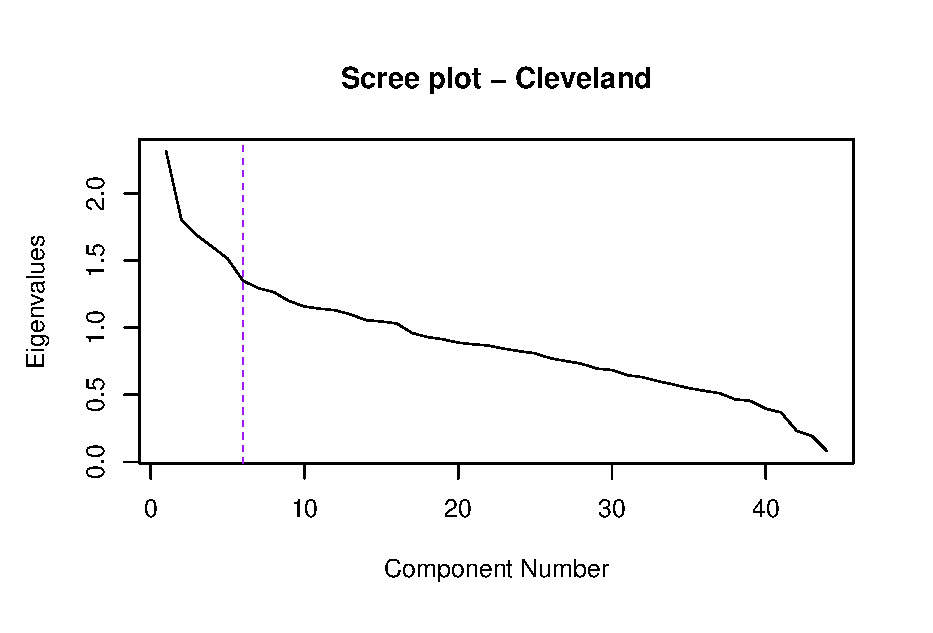
\includegraphics[width=12cm]{question3output/clescreeplot.eps}
	\end{center}
	\caption{Scree plot for PCA of Cleveland}
	\label{q3-cle-screeplot}
\end{figure}

From the scree plot in Figure \ref{q3-cle-screeplot} we see that we keep 6 components.

We have the loadings of each components as follows.

\lstinputlisting[frame=single, title={Cleveland PCA loadings}]{question3output/clepcaloadings.txt}

We see that the first principle component is mostly formed of \textbf{thaldur}, \textbf{thalach}, \textbf{met} and \textbf{oldpeak} variables.

The second principle component is mostly formed of \textbf{cyr} and \textbf{ekgyr} variables.

The third principle component is mostly formed of \textbf{tpeakbpd}, \textbf{trestbpd}, \textbf{sex} and \textbf{trestbps} variables.

The fourth principle component is mostly formed of \textbf{ekgmo} and \textbf{cmo} variables.

The fifth principle component is mostly formed of \textbf{cday}, \textbf{ekgday}, \textbf{years} and \textbf{cigs} variables.

The sixth principle component is mostly formed of \textbf{diuretic}, \textbf{htn}, \textbf{ekgday}

\subsubsection{Hungary}

After removing dummy variables and variables with at least $79\%$ NA data, we are left with 36 variables and 88 observations. 

\lstinputlisting[frame=single, title={Hungary variance inflation factor}]{question3output/hunvif.txt}

From the variance inflation factor we see that the variables \textbf{painexer}, \textbf{cp}, \textbf{ekgmo}, \textbf{ekgyr}, \textbf{proto}, \textbf{thaldur}, \textbf{thaltime}, \textbf{cmo} and \text{cyr} are highly collinear with other variables in the model.

\begin{figure}[H]
	\begin{center}
		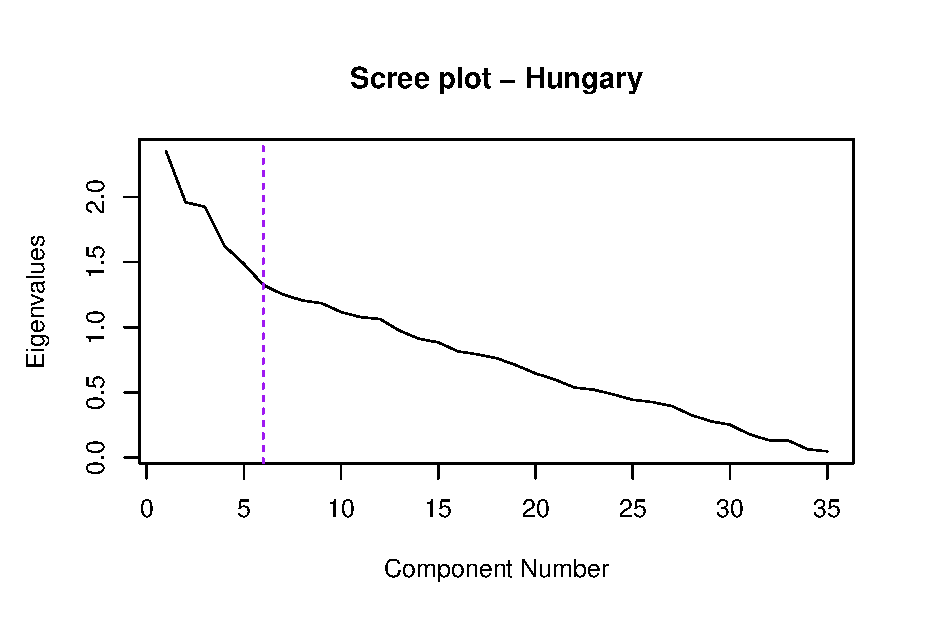
\includegraphics[width=12cm]{question3output/hunscreeplot.eps}
	\end{center}
	\caption{Scree plot for PCA of Hungary}
	\label{q3-hun-screeplot}
\end{figure}

From the scree plot in Figure \ref{q3-hun-screeplot} we see that we keep 6 components.

We have the loadings of each components as follows.

\lstinputlisting[frame=single, title={Hungary PCA loadings}]{question3output/hunpcaloadings.txt}

We see that the first principle component is mostly formed of \textbf{proto}, \textbf{met}, \textbf{thaldur} and \textbf{thaltime} variables.

The second principle component is mostly formed of \textbf{cyr}, \textbf{ekgyr} and \textbf{pro} variables.

The third principle component is mostly formed of \textbf{cp}, \textbf{painexer} and \textbf{relrest} variables.

The fourth principle component is mostly formed of \textbf{nitr} and \textbf{pro} variables.

The fifth principle component is mostly formed of \textbf{rldv5e} and \textbf{rldv5} variables.

The sixth principle component is mostly formed of \textbf{ekgday} and \textbf{cday} variables.

\subsubsection{Longbeach}

After removing dummy variables and variables with at least $50\%$ NA data, we are left with 50 variables and 94 observations.

\lstinputlisting[frame=single, title={Longbeach variance inflation factor}]{question3output/lonvif.txt}

From the variance inflation factor we see that the variables \textbf{cp}, \textbf{ekgyr}, \textbf{thaldur}, \textbf{met} and \textbf{cyr} are highly collinear with other variables in the model.

\begin{figure}[H]
	\begin{center}
		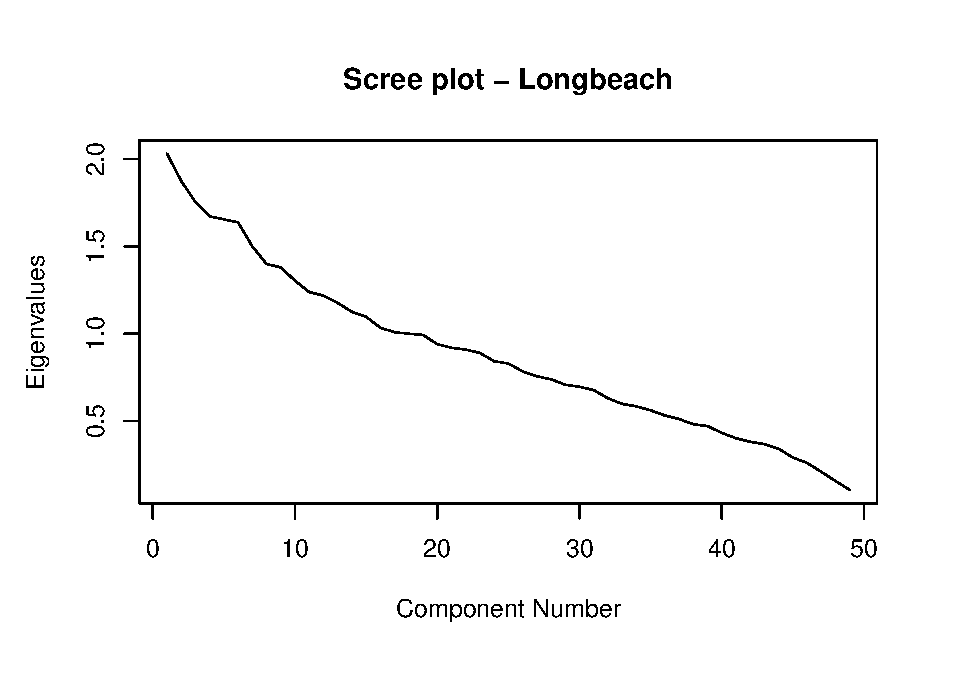
\includegraphics[width=12cm]{question3output/lonscreeplot.eps}
	\end{center}
	\caption{Scree plot for PCA of Longbeach}
	\label{q3-lon-screeplot}
\end{figure}

From the scree plot in Figure \ref{q3-lon-screeplot} we see that we keep 11 components.

We have the loadings of each components as follows.

\lstinputlisting[frame=single, title={Longbeach PCA loadings}]{question3output/lonpcaloadings.txt}

We see that the first principle component is mostly formed of \textbf{ekgyr}, \textbf{cyr} and \textbf{proto} variables.

The second principle component is mostly formed of \textbf{thaldur}, \textbf{met} variables.

The third principle component is mostly formed of \textbf{htn}, \textbf{trestbps} and \textbf{cigs} variables.

The fourth principle component is mostly formed of \textbf{years}, \textbf{smoke} and \textbf{cigs} variables.

The fifth principle component is mostly formed of \textbf{thalrest}, \textbf{thalach} and \textbf{painexer} variables.

The sixth principle component is mostly formed of \textbf{rcaprox}, \textbf{relrest} and \textbf{cp} variables.

The seventh principle component is mostly formed of \textbf{ekgday}, \textbf{rldv5} and \textbf{thalach} variables.

The eight principle component is mostly formed of \textbf{diag}, \textbf{cday} and \textbf{om2} variables.

The ninth principle component is mostly formed of \textbf{om1}, \textbf{cmo} and \textbf{ekgmo} variables.

The tenth principle component is mostly formed of \textbf{famhist}, \textbf{fbs} and \textbf{cday} variables.

The eleventh principle component is mostly formed of \textbf{ekgmo}, \textbf{trestbpd}, \textbf{cmo} and \textbf{laddist} variables.

\subsubsection{Switzerland}

After removing dummy variables and variables with at least $13\%$ NA data, we are left with 39 variables and 101 observations.

\lstinputlisting[frame=single, title={Switzerland variance inflation factor}]{question3output/swivif.txt}

From the variance inflation factor we see that the variables \textbf{ekgmo}, \textbf{ekgyr} and \textbf{cmo} are highly collinear with other variables in the model.

\begin{figure}[H]
	\begin{center}
		\includegraphics[width=12cm]{question3output/swiscreeplot.eps}
	\end{center}
	\caption{Scree plot for PCA of Switzerland}
	\label{q3-swi-screeplot}
\end{figure}

From the scree plot in Figure \ref{q3-swi-screeplot} we see that we keep 5 components.

We have the loadings of each components as follows.

\lstinputlisting[frame=single, title={Switzerland PCA loadings}]{question3output/swipcaloadings.txt}

We see that the first principle component is mostly formed of \textbf{cmo}, \textbf{ekgmo}, \textbf{ekgyr} and \textbf{cyr} variables.

The second principle component is mostly formed of \textbf{cp}, \textbf{thalrest}, \textbf{painloc}, and \textbf{painexer} variables.

The third principle component is mostly formed of \textbf{trestbps} and \textbf{age} variables.

The fourth principle component is mostly formed of \textbf{tpeakbps}, \textbf{tpeakbpd} and \textbf{oldpeak} variables.

The fifth principle component is mostly formed of \textbf{thaldur} and \textbf{laddist} variables.

\newpage
\subsection{Question 4}

In order to distinguish patients based on their disease through discriminant
analysis, I had to create four models, one for each of the datasets.

\subsubsection{Cleveland}

\lstinputlisting[frame=single]{Q4_output/q4-clev.txt}

\begin{figure}[H]
	\begin{center}
		\includegraphics[width=12cm]{Q4_pics/Clev-Histgram.png}
	\end{center}
	\caption{Histergram for discriminant analysis of Cleveland}
	\label{q4_clev_historgram}
\end{figure}

\begin{figure}[H]
	\begin{center}
		\includegraphics[width=12cm]{Q4_pics/Clev-scatter.png}
	\end{center}
	\caption{Scatter plot for discriminant analysis of Cleveland}
	\label{q4_clev_scatter}
\end{figure}

\newpage
\subsubsection{Hungary}

\lstinputlisting[frame=single]{Q4_output/Q4-hung.txt}

\begin{figure}[H]
	\begin{center}
		\includegraphics[width=12cm]{Q4_pics/Hung-Histgram.png}
	\end{center}
	\caption{Histergram for discriminant analysis of Hungary}
	\label{q4_hung_historgram}
\end{figure}

\begin{figure}[H]
	\begin{center}
		\includegraphics[width=12cm]{Q4_pics/Hung-scatter.png}
	\end{center}
	\caption{Scatter plot for discriminant analysis of Hungary}
	\label{q4_hung_scatter}
\end{figure}

\newpage
\subsubsection{Longbeach}

\lstinputlisting[frame=single]{Q4_output/Q4-long.txt}

\begin{figure}[H]
	\begin{center}
		\includegraphics[width=12cm]{Q4_pics/Long-Histgram.png}
	\end{center}
	\caption{Histergram for discriminant analysis of Longbeach}
	\label{q4_long_historgram}
\end{figure}

\begin{figure}[H]
	\begin{center}
		\includegraphics[width=12cm]{Q4_pics/Long-scatter.png}
	\end{center}
	\caption{Scatter plot for discriminant analysis of Longbeach}
	\label{q4_long_scatter}
\end{figure}

\newpage
\subsubsection{Switzerland}

\lstinputlisting[frame=single]{Q4_output/Q4-swit.txt}

\begin{figure}[H]
	\begin{center}
		\includegraphics[width=12cm]{Q4_pics/Swit-Histgram.png}
	\end{center}
	\caption{Histergram for discriminant analysis of Switzerland}
	\label{q4_swit_historgram}
\end{figure}

\begin{figure}[H]
	\begin{center}
		\includegraphics[width=12cm]{Q4_pics/Swit-scatter.png}
	\end{center}
	\caption{Scatter plot for discriminant analysis of Switzerland}
	\label{q4_swit_scatter}
\end{figure}

\section{Summary}

\end{document}
